\documentclass[12pt]{article}

% Basic packages only
\usepackage[margin=1in]{geometry}
\usepackage{graphicx}
\usepackage{amsmath}
\usepackage{booktabs}
\usepackage{setspace}
\usepackage{hyperref}
\usepackage{float}

\begin{document}
% \onehalfspacing
\doublespacing

% Front matter uses roman numerals
\pagenumbering{roman}

% ── TITLE PAGE ────────────────────────────────────────────────────
\begin{titlepage}
  \centering
  \thispagestyle{empty}

  {\large Loyola Marymount University, Los Angeles, California}

  \vspace{1.5cm}

  {\Huge\bfseries
    Hybrid Rendering: Combining Ray-Tracing\\[6pt]
    with Static Techniques as Applied to\\[6pt]
    Rendering Stained Glass
  }

  \vspace{1.5cm}

  {A thesis submitted in partial satisfaction of the requirements for the degree Master of Science in Computer Science}

  \vspace{1.5cm}

  {by}\\[8pt]
  {\LARGE\bfseries Matthew Lee}

  \vfill

  {April 2026}
\end{titlepage}

% ── COMMITTEE APPROVAL ────────────────────────────────────────────
\clearpage
\section*{Approval Page}

The thesis of Matthew Lee is approved.

\vspace{2cm}
\noindent\underline{\hspace{8cm}}\\[4pt]
Dr.\ Ray Toal, Thesis Advisor

\vspace{1.5cm}
\noindent\underline{\hspace{8cm}}\\[4pt]
Committee Member

\vspace{1.5cm}
\noindent\underline{\hspace{8cm}}\\[4pt]
Committee Member

% ── ABSTRACT ──────────────────────────────────────────────────────
\clearpage
\section*{Abstract}

Real-time rendering pipelines must balance visual fidelity against computational cost. This thesis presents a hybrid rendering approach that combines pre-baked static lightmaps for the stationary window panel with a dynamic screen-space refraction shader for GPU-instanced boid agents. The stationary window panel uses a UV-mapped source texture augmented by Spherical Harmonics ambient lighting, Fresnel reflection, and screen-space refraction. The technique is demonstrated through a Unity Universal Render Pipeline (URP) implementation applied to a GPU-instanced boid simulation rendered against a stained-glass window. Performance measurements across four agent populations (100, 250, 500, and 1000 boids) reveal that all three configurations perform comparably at low agent counts, but diverge sharply at scale: the static configuration degrades to 11.38\,ms at 1000 boids while the hybrid and dynamic configurations hold at 3.71\,ms and 4.66\,ms respectively. The results demonstrate that assigning shader configurations per object class --- static lightmap for stationary geometry and a lightweight refraction-and-tint shader for GPU-instanced agents --- is not only practically viable but constitutes the most GPU-efficient strategy at scale, delivering equivalent or superior frame cost to a purely dynamic pipeline at every tested agent count.

% ══════════════════════════════════════════════════════════════════
% Table of Contents
% ══════════════════════════════════════════════════════════════════
\clearpage
\tableofcontents

% ── ACKNOWLEDGEMENTS ──────────────────────────────────────────────
\clearpage
\section*{Acknowledgements}

Many thanks to Dr.\ Ray Toal for his invaluable guidance and mentorship throughout the development of this thesis. Gratitude is also extended to fellow project members Grayson von Goetz und Schwanenfleiss and Clifford Phillips for their thoughtful contributions to the overall project.

% Switch to arabic numbering for the body
\clearpage
\pagenumbering{arabic}

% ══════════════════════════════════════════════════════════════════
% SECTION 1: INTRODUCTION
%══════════════════════════════════════════════════════════════════
\clearpage
\section{Introduction}


Hybrid rendering approaches are not a new technology, particularly within game rendering pipelines. Conventional approaches partition a scene's lighting workload by assigning each technique to the geometry for which it is best suited: pre-baked static lighting for geometry whose illumination conditions are fixed at authoring time, and fully dynamic runtime lighting for geometry that moves or whose environment changes each frame.

Real-time rendering pipelines must balance visual fidelity against computational cost. Two canonical strategies --- static pre-baked lighting and fully dynamic runtime lighting --- each offer distinct trade-offs that make neither sufficient on its own for scenes containing both stationary geometry and rapidly moving agents such as boids.

Static lighting utilizes pre-computed, or baked, lightmaps in order to impose negligible runtime overhead ($\approx 0.1\,\text{ms}$ per frame), since illumination data is stored before runtime in the applied textures, and retrieved later when called. However, since baking is a process which must be completed before compiling, this approach becomes unviable for fast moving objects, whose lighting data would ideally be calculated during runtime.

Dynamic lighting, on the other hand, is fully responsive to environment changes, but carries a cost which scales with the rate of positional change of each object. However, for GPU-instanced agents such as boids, which may number in the hundreds to thousands and \textbf{must} update their position each frame, fully dynamic lighting can be extremely computationally costly. Additionally, dynamic lighting generally struggles to match the same level of detail that a pre-rendered lightmap can achieve.

The central thesis of this work is that assigning each rendering strategy to the object class for which it is appropriate --- a UV-mapped source-texture shader augmented by runtime Spherical Harmonics, Fresnel reflection, and screen-space refraction for the stationary window panel, and a lightweight screen-space refraction shader tinted by the source image for GPU-instanced boid agents --- is not only technically viable but constitutes the most GPU-efficient strategy at scale, with minimal visual trade-offs relative to a purely static or purely dynamic pipeline.

This will be demonstrated through a Unity Universal Rendering Pipeline (URP) implementation that applies \texttt{StainedGlassShader.shadergraph} to the stationary stained-glass window panel and \texttt{StainedGlassShaderDynamic.shadergraph} to C.J.\ Phillips' GPU-instanced boid agents, comparing the hybrid configuration against static and fully dynamic baselines.

The rest of this thesis is organized as follows. Section~\ref{sec:background} surveys relevant prior work, including distributed hybrid rendering, spherical harmonics lighting, boid simulation, and light probes. Section~\ref{sec:methods} describes the hybrid pipeline design and implementation. Section~\ref{sec:tradeoffs} analyzes the trade-offs among the three rendering configurations. Section~\ref{sec:performance} presents performance measurements and analysis. The thesis concludes with a summary of results, limitations, and directions for future research.

% ══════════════════════════════════════════════════════════════════
% SECTION 2: BACKGROUND
% ══════════════════════════════════════════════════════════════════
\clearpage
\section{Background and Related Work}
\label{sec:background}

This section details both relevant work which is related to hybrid rendering techniques, as well as a brief background into boid simulations. 

% ══════════════════════════════════════════════════════════════════
% Hybrid Rendering
% ══════════════════════════════════════════════════════════════════
\subsection{Distributed Hybrid Rendering with Real-Time Shadows (DHR+S)}
\label{subsec:dhrs}
 
Tan et al.\ \cite{TanLowChow2024} present DHR+S, an extension of their earlier Distributed Hybrid Rendering (DHR) framework targeting thin clients such as standalone extended-reality headsets and mobile devices. The central premise of DHR is a division of rendering labour: rasterization runs locally on the client while computationally expensive ray tracing is offloaded to a remote server, with the ray-traced output streamed back over a network connection. DHR+S augments this baseline by adding two shadow-quality improvements --- ray-traced soft shadows and filtered ambient occlusion --- without substantially increasing bandwidth consumption.
 
Soft shadows are produced by introducing bounded directional variance to each shadow ray so that it samples the full emitting surface area of a light source rather than a single central point. For pixels near the silhouettes of occluding objects this produces partial occlusion, yielding a physically plausible penumbra. Ambient occlusion is approximated by casting a small hemisphere of rays from each surface point and computing the fraction that remain unoccluded; only a single byte per pixel is transmitted to encode this value.
 
Because stochastic ray sampling introduces noise at low ray counts, the authors apply a modified version of Spatiotemporal Variance-Guided Filtering (SVGF) \cite{Schied2017}, adapted to use depth and normal differentials rather than luminance as the variance signal.
 
This work is directly relevant to the hybrid rendering strategy explored in this thesis. In particular, the DHR+S treatment of the dynamic--static rendering boundary --- performing expensive ray-traced passes remotely while delegating locally computable rasterization to the client --- mirrors the motivation behind the static-to-dynamic lighting transitions described in Section~\ref{sec:methods}. Where DHR+S distributes the workload spatially across a network, the approach presented here addresses the same fidelity--cost trade-off within a single GPU through selective application of a UV-mapped source texture with Spherical Harmonics and Fresnel reflection for the stationary window panel, and a lightweight screen-space refraction shader for GPU-instanced boid agents.

% ══════════════════════════════════════════════════════════════════
% Boids
% ══════════════════════════════════════════════════════════════════
\subsection{Boids and GPU-Instanced Crowd Simulation}
The boid model, originally introduced by Reynolds \cite{Reynolds1987}, simulates the emergent flocking behavior of birds through three local steering rules applied independently to each agent: \textit{separation}, which prevents agents from colliding with neighbors; \textit{alignment}, which steers each agent toward the average heading of its local group; and \textit{cohesion}, which pulls each agent toward the average position of its neighbors. Despite the simplicity of these rules, the aggregate behavior of a large population produces convincingly lifelike flocking motion.
The computational challenge of boid simulation arises from neighbor search: in a naive implementation, each boid must be tested against every other, yielding $O(n^2)$ complexity that quickly becomes prohibitive at scale. GPU implementations address this by encoding boid state --- position, orientation, and force --- into texture maps and performing simulation entirely on the GPU, with a uniform spatial grid used to accelerate neighbor lookups to sub-linear complexity \cite{Silva2008}. At population sizes of tens of thousands of agents, fully GPU-resident simulation and rendering becomes not only feasible but necessary for real-time performance.

This project applies the custom stained-glass shaders to the boid simulation developed by C.J. Phillips. Because boids are rendered via GPU instancing --- where a single draw call renders all agents using shared mesh data --- each agent lacks a unique secondary UV channel (\texttt{UV2}), which Unity requires to sample a per-object pre-baked lightmap. This structural constraint motivates the use of a custom shader for the boid agents that carries no lightmap dependency, as described in Sections~\ref{subsec:hybrid-strategy} and~\ref{subsec:technical-components}.

% ══════════════════════════════════════════════════════════════════
% Spherical Harmonics
% ══════════════════════════════════════════════════════════════════

\subsection{Spherical Harmonics}
Spherical Harmonics --- specifically the nine-coefficient \emph{SH9} basis --- encode incoming radiance at a point across all directions without requiring UV-mapped geometry, making them well-suited for per-object lighting of geometry that cannot carry lightmap UVs \cite{Green2003}.
A key limitation of SH is their inability to represent high-frequency lighting detail with a small coefficient budget. In practice, the diffuse contribution is well-captured by just a few low-order bands, since the clamped cosine lobe that models Lambertian reflectance concentrates most of its energy in the lowest frequencies. However, restricting diffuse computation to only three SH bands introduces visible ringing artifacts, particularly when illumination is strongly directional \cite{Mezieres2021}.
SH are evaluated at runtime via a custom HLSL function \texttt{SampleSH\_float} (defined in \texttt{SampleSH.hlsl}), exposed in Shader Graph as a Custom Function node. The function reads the seven four-component per-object coefficient arrays (\texttt{unity\_SHAr} through \texttt{unity\_SHC}) directly from Unity's constant buffers and passes them to \texttt{SampleSH9} internally, providing a spatially-varying but computationally cheap estimate of the environmental irradiance at the surface normal of the shaded fragment. In this project, SH evaluation is used in the hybrid window-panel shader (\texttt{StainedGlassShader.shadergraph}) to provide ambient lighting for the stationary window panel, as described in Section~\ref{sec:methods}.

% ══════════════════════════════════════════════════════════════════
% Light Probes
% ══════════════════════════════════════════════════════════════════
\subsection{Light Probes}
\label{subsec:light-probes}

Light probes are point samples of the incident radiance field stored at
fixed positions in the scene, typically arranged in a sparse
three-dimensional grid and baked during a precomputation stage. At
runtime, each probe's cached radiance is queried and interpolated to
produce an estimate of indirect illumination at arbitrary world-space
positions --- including positions belonging to dynamic or GPU-instanced
geometry that cannot carry its own lightmap UVs. In this sense light
probes occupy an intermediate position on the static--dynamic rendering
spectrum: the probe data itself is pre-baked, but the sampling and
interpolation that produce a final per-object shading value occur
entirely at runtime.

Classical probe formulations encode only low-frequency diffuse
irradiance --- typically as a small set of spherical-harmonic
coefficients per probe --- which is sufficient for soft ambient
shading but cannot reproduce glossy reflections, parallax-correct
highlights, or multi-bounce global illumination. Guo et al.\
\cite{Guo2022} address these limitations directly in \emph{Efficient
Light Probes for Real-Time Global Illumination}, a probe-based pipeline
that extends the expressiveness of baked probe data while retaining
real-time performance. Rather than storing only irradiance, their probes
cache full radiance information which is then reprojected to arbitrary
query viewpoints using a gradient-based search procedure. The search
converges quickly to the correct reprojected sample and, unlike
nearest-probe or trilinear-weighted lookups, does not introduce the
parallax errors that typically manifest as drifting highlights or
misaligned reflections when a shaded point lies far from the sampled
probe positions.

To compensate for the limited spatial resolution of a sparse probe grid
and the potentially low per-probe sampling rate, Guo et al.\ pair the
reprojection step with a lightweight neural image-reconstruction network
that consumes several G-buffers (surface normals, depth, material
identifiers) alongside the reprojected probe samples to synthesise a
high-resolution output. A temporal reprojection strategy and an explicit
temporal loss term during training suppress flicker across animation
sequences. The complete pipeline sustains real-time performance
(above 30 frames per second at $1920 \times 1080$) while reproducing
glossy reflections with multiple indirect bounces --- effects that are
normally the exclusive domain of fully dynamic path tracing.

The relevance of this work to the present thesis is twofold. First, it
reinforces that the boundary between ``static'' and ``dynamic'' lighting
is not a binary one: probe-based methods occupy a middle ground in which
baked data is re-interpreted each frame to serve dynamic shading needs,
exactly the philosophy driving the hybrid pipeline in
Section~\ref{sec:methods}. Second, the design trade-offs that Guo et al.\ identify --- among probe storage, reprojection accuracy, and runtime reconstruction cost --- directly inform the choice to use SH9 probes in the window-panel shader rather than a denser radiance-probe representation: the stationary panel occupies a fixed world-space position and low-frequency ambient irradiance is sufficient for its shading needs, making the lightweight \texttt{SampleSH9} call an appropriate fit without incurring the cost of the full neural reconstruction pipeline.


% ══════════════════════════════════════════════════════════════════
% SECTION 3: METHODS
% ══════════════════════════════════════════════════════════════════
\clearpage
\section{Methods}
\label{sec:methods}
 
\subsection{Problem Formulation}
\label{subsec:problem-formulation}

The rendering challenge in this work arises from a structural incompatibility between the two object classes in the scene: a stationary stained-glass window panel and a large population of GPU-instanced boid agents representing individual glass shards in flight.

The static window panel is a single mesh with unique UV coordinates (\texttt{UV0}). It can be assigned a fixed source-image texture that is mapped once at scene load and sampled every frame with negligible cost. Its fixed world-space position makes it a natural candidate for Spherical Harmonics ambient lighting evaluated at the panel's surface normal, as provided by the window-panel shader.

The boid glass shards present a different constraint. Because all boid meshes are rendered in a single GPU-instanced draw call, every agent shares identical mesh data and therefore lacks a unique secondary UV channel (\texttt{UV2}), which Unity requires to sample a per-object pre-baked lightmap. A standard URP material applied to GPU-instanced boids with no lightmap UVs causes Unity to fall back to a per-draw-call probe blending and shader-variant switching path --- overhead that scales unfavourably with agent count. Furthermore, the shards move through the scene each frame, so a pre-baked illumination solution cannot capture their changing visual environment.

The hybrid configuration resolves this incompatibility by assigning each rendering strategy to the object class for which it is appropriate: the hybrid window-panel shader (\texttt{StainedGlassShader.shadergraph}) with UV-mapped texture, Spherical Harmonics ambient lighting, Fresnel reflection, and screen-space refraction for the static panel, and a lightweight refraction-and-tint shader (\texttt{StainedGlassShaderDynamic.shadergraph}) for the instanced boid shards.

\subsection{Pipeline Overview}
\label{subsec:hybrid-strategy}

The pipeline is implemented using two custom Unity Shader Graph assets and one standard URP material, compiled into three distinct rendering configurations.

In the \emph{static} configuration, all geometry --- the window panel and every boid agent --- uses \texttt{StainedGlassStatic.mat}, a plain Unity URP material carrying a pre-baked \texttt{BaseMap} texture and a \texttt{BumpMap}. No custom shader graph is involved; illumination is encoded entirely in the baked texture data. In the \emph{dynamic} configuration, all geometry uses \texttt{StainedGlassShaderDynamic.shadergraph}, a custom shader that applies screen-space refraction --- sampling the scene behind the glass using a \texttt{DistortionText}-warped screen UV --- and tints the result by multiplying with the \texttt{MainText} source image. This gives each boid position-dependent visual variation (the refracted scene differs per screen position) while sharing the same source-image colour palette as the static window.

The \emph{hybrid} configuration assigns each shader to the object class for which it is appropriate: the stationary window panel uses \texttt{StainedGlassShader.shadergraph}, a texture-based shader that maps a source image onto the glass surface and augments it with screen-space refraction, Fresnel reflection, Spherical Harmonics ambient lighting, and a Saturation post-process. The GPU-instanced boid glass shards use \texttt{StainedGlassShaderDynamic.shadergraph}, which applies the same refraction-and-tint approach without the Fresnel, Spherical Harmonics, or Saturation stages. A transitional material (\texttt{HybridShader.mat}) handles geometry at the window boundary.

The three rendering paths are described in Sections~\ref{subsec:static-path}, \ref{subsec:hybrid-window-path}, and~\ref{subsec:dynamic-path}.

\subsection{Static Rendering Path}
\label{subsec:static-path}

In the static configuration, \texttt{StainedGlassStatic.mat} is applied uniformly to all geometry --- the window panel and all boid agents alike. This is a standard Unity URP material with no custom Shader Graph; it carries a pre-baked \texttt{BaseMap} (the source stained-glass image) and a \texttt{BumpMap} for surface micro-detail. All illumination information is encoded offline into the baked texture; at runtime the material simply samples these textures with negligible cost. 

The limitation of this approach for GPU-instanced boid agents is structural: because all instances share identical mesh data, none can carry a unique secondary UV channel (\texttt{UV2}) required to sample a per-object lightmap. Unity's fallback for un-baked GPU-instanced geometry involves per-draw-call probe blending and additional shader variant switching, overhead that scales unfavourably with agent count and is the primary driver of the static configuration's degradation at 1000 boids (see Section~\ref{sec:performance}).

\subsection{Dynamic Rendering Path}
\label{subsec:dynamic-path}

The dynamic path is implemented in \texttt{StainedGlassShaderDynamic.shadergraph}. It exposes four material properties: \texttt{\_MainText} (the source image), \texttt{\_DistortionText} (a warp texture), \texttt{\_Normal} (a surface normal map), and \texttt{\_NormalIntensity} (a scalar).

\subsubsection{Screen-Space Refraction}

The core visual effect is screen-space refraction. A \textbf{Screen Position} node supplies the fragment's current screen UV. A \textbf{Normal Vector} node (world space) and a sample of \texttt{\_DistortionText} are combined via an Add and two Multiply nodes to produce a UV offset; this offset is added to the screen UV and passed to a \textbf{Scene Color} node, which reads the colour of whatever scene geometry lies behind the glass surface at that displaced coordinate. The result is a physically plausible transmissive distortion: objects behind each boid shard appear warped according to the normal map and distortion texture.

\subsubsection{Texture Tint and Base Color}

The refracted scene colour is then element-wise multiplied by a sample of \texttt{\_MainText} taken at the mesh's UV0 coordinates. This multiply tints the refracted background with the colour palette of the source image, giving each shard the appearance of a coloured glass fragment. Because boids share mesh data, all instances sample the same UV point on \texttt{\_MainText}; per-instance visual variation therefore arises entirely from the screen-space position of each shard (which determines what lies behind it and thus what the refraction reveals). The result feeds into the \textbf{Base Color} output. The alpha channel of the \texttt{\_MainText} sample is separately routed to the \textbf{Occlusion} output.

Note that the shader graph file also contains two \textbf{Voronoi} nodes connected through a \textbf{Blend} node; this sub-network is entirely disconnected from the \textbf{Base Color} or any other output and does not contribute to the rendered result.


\subsection{Hybrid Window-Panel Shader Path}
\label{subsec:hybrid-window-path}

In the hybrid configuration, the stationary window panel uses \texttt{StainedGlassShader.shadergraph}, which computes the final fragment colour through four concurrent contributions. It exposes six material properties: \texttt{\_MainText}, \texttt{\_DistortionText}, \texttt{\_Normal}, \texttt{\_NormalPower}, \texttt{\_Saturation}, and \texttt{\_FresnelPower}.

First, the source image (\texttt{MainText}) is sampled at the mesh's \texttt{UV0} coordinates to obtain the glass colour pattern. A separate distortion texture (\texttt{DistortionText}) warps the screen-space UV coordinates before sampling Unity's \texttt{Scene Color} node, producing a transmissive refraction effect in which the scene behind the glass is visible with a colour-dependent warp. Surface micro-detail is added via a \texttt{Normal} map attenuated by \texttt{NormalPower}.

Second, a \textbf{Fresnel Effect} node modulates view-dependent reflectivity at glancing angles, with intensity controlled by \texttt{FresnelPower}. A \textbf{One Minus} node inverts the Fresnel factor so that grazing-angle fragments attenuate the refraction contribution rather than add to it.

Third, the Spherical Harmonics ambient contribution is evaluated via the custom inline HLSL function \texttt{SampleSH} (defined in \texttt{SampleSH.hlsl}), exposed in Shader Graph as a Custom Function node:

\begin{verbatim}
void SampleSH_float(float3 WorldNormal, out float3 Color)
{
    real4 SHCoefficients[7];
    SHCoefficients[0] = unity_SHAr;  // L1 red
    SHCoefficients[1] = unity_SHAg;  // L1 green
    SHCoefficients[2] = unity_SHAb;  // L1 blue
    SHCoefficients[3] = unity_SHBr;  // L2 red
    SHCoefficients[4] = unity_SHBg;  // L2 green
    SHCoefficients[5] = unity_SHBb;  // L2 blue
    SHCoefficients[6] = unity_SHC;   // L2 shared
    Color = max(float3(0,0,0),
                SampleSH9(SHCoefficients, WorldNormal));
}
\end{verbatim}

The function reads Unity's per-object SH coefficient arrays and evaluates the SH9 basis against the panel's world-space normal, providing a low-frequency estimate of indirect irradiance without requiring UV-mapped lightmap data. This SH output is combined with the refracted scene colour via Multiply nodes.

Fourth, two \textbf{Saturation} nodes post-process the sampled scene colour, allowing artists to control the intensity of the colour cast. The final combined result is output to \textbf{Base Color}.


\subsection{Technical Components}
\label{subsec:technical-components}

All shading logic is authored in Unity's Shader Graph visual programming environment targeting the Universal Render Pipeline (URP). Shader Graph compiles the node graph to HLSL at build time, ensuring compatibility with URP's render passes. The computationally non-trivial operation in the window-panel shader --- SH evaluation --- is expressed as a Custom Function node containing inline HLSL so that it can directly access Unity's per-object constant buffers (\texttt{unity\_SHAr} through \texttt{unity\_SHC}) that are not exposed as standard Shader Graph nodes.

The window-panel shader (\texttt{StainedGlassShader.shadergraph}) exposes the following artist-facing properties:
\begin{itemize}
  \item \texttt{MainText} --- the source image texture mapped onto the glass surface.
  \item \texttt{DistortionText} --- a distortion texture that warps screen-space UVs to produce the refraction offset.
  \item \texttt{Normal} --- a surface normal map applied via a \texttt{Normal Strength} node.
  \item \texttt{NormalPower} --- scalar controlling the influence of the normal map.
  \item \texttt{Saturation} --- post-processes the saturation of the sampled scene colour.
  \item \texttt{FresnelPower} --- controls the intensity of view-dependent Fresnel reflection.
\end{itemize}

The dynamic shader (\texttt{StainedGlassShaderDynamic.shadergraph}) exposes a reduced set of properties: \texttt{MainText}, \texttt{DistortionText}, \texttt{Normal}, and \texttt{NormalIntensity}. It omits the Fresnel, SH, and Saturation stages present in the window-panel shader.

The \texttt{ImageToGlassPipeline} C\# component assigns the correct source image texture to both shaders at scene load time by setting \texttt{mat.mainTexture} and the shader's \texttt{maintext} property slot.

% ══════════════════════════════════════════════════════════════════
% SECTION 4: TRADE-OFFS
% ══════════════════════════════════════════════════════════════════
\clearpage
\section{Trade-offs Between Rendering Approaches}
\label{sec:tradeoffs}

The three rendering configurations examined in this work --- static lightmap, fully dynamic screen-space refraction, and hybrid --- each occupy a distinct position in the fidelity-versus-cost design space. This section analyses the qualitative and quantitative trade-offs among them, illustrated by representative renders of the stained-glass panel under each approach.

\subsection{Static Lightmap Rendering}

\begin{figure}[H]
  \centering
  \includegraphics[width=0.55\textwidth]{Static.png}
  \caption{Static lightmap rendering of the stained-glass window panel. Pre-baked illumination yields rich, high-fidelity colour and shadow detail at negligible runtime cost.}
  \label{fig:static}
\end{figure}

As shown in Figure~\ref{fig:static}, the static lightmap approach produces the richest colour saturation and most detailed shadow distribution of the three configurations. Because the entire illumination solution is computed offline, the baker can afford to use a high sample count, multi-bounce global illumination, and fine texel resolution without any real-time budget constraint. The resulting render exhibits accurate coloured light bleeding between adjacent glass panes and smooth penumbrae at the lead came edges.

The fundamental limitation of this approach is its inability to respond to runtime changes. Any moving object --- including the boid glass shards --- cannot carry baked lightmap data, since GPU instancing precludes unique \texttt{UV2} assignments per agent. Furthermore, any modification to scene geometry or lighting that occurs after the bake step requires a full rebake, which may take several minutes even for moderately complex scenes. The static approach is therefore best suited to geometry that is guaranteed not to move and for which illumination conditions are fixed at authoring time.


\subsection{Fully Dynamic Rendering}

\begin{figure}[H]
  \centering
  \includegraphics[width=0.55\textwidth]{Dynamic.png}
  \caption{Fully dynamic rendering using screen-space refraction and MainText texture tinting. The scene behind each boid is visible through the glass surface, producing position-dependent colour variation across the agent population.}
  \label{fig:dynamic}
\end{figure}

The dynamic configuration, illustrated in Figure~\ref{fig:dynamic}, replaces the pre-baked lightmap with a screen-space refraction pass tinted by the source image. This approach is compatible with GPU-instanced geometry: because the refraction reads from the screen at each fragment's position and the texture tint is applied at shared UV coordinates, neither operation requires unique per-instance UV channels. Boids therefore receive position-dependent visual variation --- each shard refracts the scene geometry visible behind it --- without a per-instance lightmap bake.

The visual trade-off is visible in Figure~\ref{fig:dynamic}: the colour gradients across the boid population are determined by what each shard refracts rather than by a high-resolution baked illumination solution. Fine-grained variation within individual glass panes is absent compared to the static render. Measured mean GPU costs range from $2.02\,\text{ms}$ at 100 agents to $4.66\,\text{ms}$ at 1000 agents. Critically, this cost grows only modestly with agent count --- a factor of roughly $2.3\times$ from 100 to 1000 boids --- because the screen-space refraction and texture lookup are $O(1)$ per fragment and therefore scale with rasterised area rather than agent count.

A dynamic approach is compatible with GPU-instanced objects; per-frame GPU cost scales with agent count; produces lower colour fidelity and loss of high-frequency lighting detail relative to a baked solution, but is fully responsive to the scene geometry visible through the glass surface.

\subsection{Hybrid Rendering}

\begin{figure}[H]
  \centering
  \includegraphics[width=0.55\textwidth]{Hybrid.png}
  \caption{Hybrid rendering combining the UV-texture window-panel shader (with Spherical Harmonics, Fresnel, and screen-space refraction) for the stationary window with the lightweight refraction-and-tint shader for GPU-instanced boid agents.}
  \label{fig:hybrid-render}
\end{figure}

The hybrid approach, shown in Figure~\ref{fig:hybrid-render}, assigns each shader to the object class for which it is appropriate. The static window panel uses the hybrid window-panel shader (\texttt{StainedGlassShader.shadergraph}) with its UV-mapped texture, screen-space refraction, Fresnel reflection, Spherical Harmonics ambient lighting, and Saturation post-process, while the boid agents use \texttt{StainedGlassShaderDynamic.shadergraph} with the lightweight refraction-and-tint pipeline. A transitional material (\texttt{HybridShader.mat}) handles geometry at the boundary between the two object classes.

Comparing Figure~\ref{fig:hybrid-render} with Figures~\ref{fig:static} and~\ref{fig:dynamic} reveals the practical result of this strategy: the window panel itself benefits from the richer window-panel shader (SH, Fresnel, Saturation), while the boid agents receive the same screen-space refraction and texture tinting as in the fully dynamic configuration. Measured GPU cost for the hybrid configuration is comparable to or lower than the fully dynamic configuration at every tested agent count, and at 1000 boids is less than one-third the cost of the purely static configuration (see Section~\ref{sec:performance}).

The primary limitation of the hybrid approach is authoring complexity: the scene must contain both a correctly UV-unwrapped static mesh and two properly configured shader assets with matching material properties. The window-panel shader requires light probes to be baked in the scene for the SH contribution to be meaningful. Scenes with multiple stained-glass windows or complex multi-directional lighting would require additional authoring effort to ensure the SH and Fresnel contributions are correctly calibrated.

A hybrid rendering approach combines the high fidelity of static baking for stationary geometry with the runtime flexibility of dynamic lighting for GPU-instanced agents; minimal additional per-frame overhead relative to the purely dynamic configuration; requires a precomputation pass for the static component and additional authoring setup.

% ══════════════════════════════════════════════════════════════════
% SECTION 5: PERFORMANCE ANALYSIS
% ══════════════════════════════════════════════════════════════════
\clearpage
\section{Performance Analysis}
\label{sec:performance}

Tests were performed on a Mac with the following specifications:
\begin{itemize}
  \item Processor: Apple M2
  \item Memory: 16\,GB RAM
  \item Graphics Processor: Apple M2 (unified memory)
  \item Unity Version: 6000.3.8f1
\end{itemize}
All times are in milliseconds. Each configuration was profiled in isolation within Unity's Play mode; GPU frame time was recorded via \texttt{ProfilerRecorder} over approximately 30 seconds per run after discarding the first 30 warmup frames.

\subsection{Per-Frame GPU Cost}

Table~\ref{tab:frame-cost} summarises the per-frame GPU cost for each lighting configuration across four agent populations. Four boid counts were chosen to span the practical range of the simulation: 100 agents (low load), 250 (moderate), 500 (high), and 1000 (stress test).

\begin{table}[htbp]
  \centering
  \caption{Measured per-frame GPU cost by rendering configuration and boid count. Values are mean~$\pm$~1\,s.d.\ over recorded frames. Hardware: Apple M2, 16\,GB RAM, Unity 6000.3.8f1.}
  \label{tab:frame-cost}
  \begin{tabular}{llccccc}
    \toprule
    \textbf{Configuration} & \textbf{Boids} & \textbf{Mean (ms)} & \textbf{Std (ms)} & \textbf{Min (ms)} & \textbf{Max (ms)} & \textbf{p95 (ms)} \\
    \midrule
    Static & 100 & 2.02 & 0.33 & 0.40 & 5.73 & 2.42 \\
    Static & 250 & 4.10 & 0.48 & 2.23 & 17.12 & 4.27 \\
    Static & 500 & 4.06 & 0.95 & 1.12 & 12.51 & 5.66 \\
    Static & 1000 & 11.38 & 1.65 & 0.44 & 13.78 & 12.47 \\
    Dynamic & 100 & 2.02 & 0.34 & 0.39 & 8.02 & 2.34 \\
    Dynamic & 250 & 4.06 & 0.48 & 0.56 & 16.15 & 4.46 \\
    Dynamic & 500 & 3.78 & 1.49 & 0.10 & 23.65 & 5.86 \\
    Dynamic & 1000 & 4.66 & 1.54 & 0.77 & 15.26 & 7.85 \\
    Hybrid & 100 & 1.97 & 0.44 & 0.13 & 20.59 & 2.30 \\
    Hybrid & 250 & 4.13 & 0.79 & 0.10 & 13.08 & 4.35 \\
    Hybrid & 500 & 3.90 & 0.41 & 0.10 & 8.67 & 4.15 \\
    Hybrid & 1000 & 3.71 & 0.92 & 0.11 & 11.49 & 4.58 \\
    \bottomrule
  \end{tabular}
\end{table}

The data reveal three distinct performance regimes.

At 100 boids, all three configurations are statistically indistinguishable: means of 2.02\,ms (Static), 2.02\,ms (Dynamic), and 1.97\,ms (Hybrid). At this agent count the per-boid contribution to frame time is small relative to fixed scene overhead --- camera setup, shadow passes, and scene rendering --- and the choice of boid shader has no measurable impact.

At 250--500 boids, all three configurations remain closely matched, with means in the $3.78$--$4.13\,\text{ms}$ range. The Static configuration's standard deviation widens at 500 boids (0.95\,ms versus 0.48\,ms at 250), suggesting that Unity's batching heuristics begin to produce occasional frame spikes as the instanced draw call grows. Dynamic and Hybrid costs rise gradually but remain within $0.35\,\text{ms}$ of each other across this range.

At 1000 boids, the configurations diverge sharply. Static cost jumps to $11.38\,\text{ms}$ (mean) with a p95 of $12.47\,\text{ms}$, indicating that this elevated cost is sustained rather than spike-driven. Dynamic holds at $4.66\,\text{ms}$ and Hybrid at $3.71\,\text{ms}$ --- a $2.4\times$ and $3.1\times$ advantage over Static respectively.

The Static configuration's degradation at scale is the most consequential finding of this study. Although the pre-baked lightmap itself incurs negligible sampling cost, Unity's GPU-instancing path for the boid agents cannot use per-instance lightmap UVs. At large agent counts, the engine's fallback lighting path for these un-baked instances --- which involves per-draw-call probe blending and additional shader variant switching --- introduces overhead that scales unfavourably with agent count. The Dynamic and Hybrid configurations avoid this by design: the custom boid shader (\texttt{StainedGlassShaderDynamic.shadergraph}) has no lightmap dependency and resolves all per-fragment work --- screen-space refraction and texture sampling --- uniformly within a single shader variant, preserving Unity's batching efficiency at 1000 agents and beyond.

\subsection{Scaling and Time-Series Analysis}

\begin{figure}[H]
  \centering
  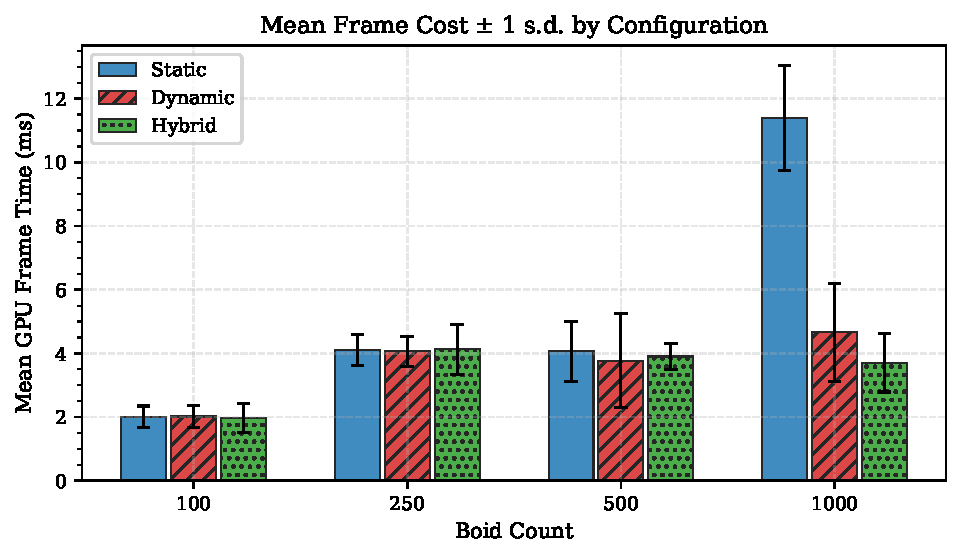
\includegraphics[width=0.55\textwidth]{profiler_barchart.jpg}
  \caption{Mean GPU frame cost ($\pm$1\,s.d.) per rendering configuration and boid count.}
  \label{fig:perf-bar}
\end{figure}

\begin{figure}[H]
  \centering
  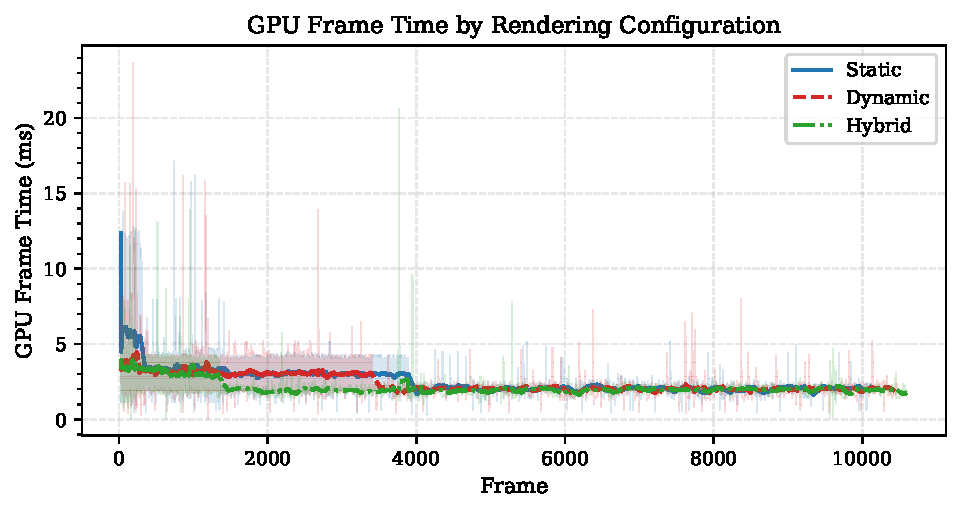
\includegraphics[width=0.55\textwidth]{profiler_timeseries.jpg}
  \caption{Rolling-average GPU frame time per configuration over the recording period (all boid counts overlaid).}
  \label{fig:perf-ts}
\end{figure}

\begin{figure}[H]
  \centering
  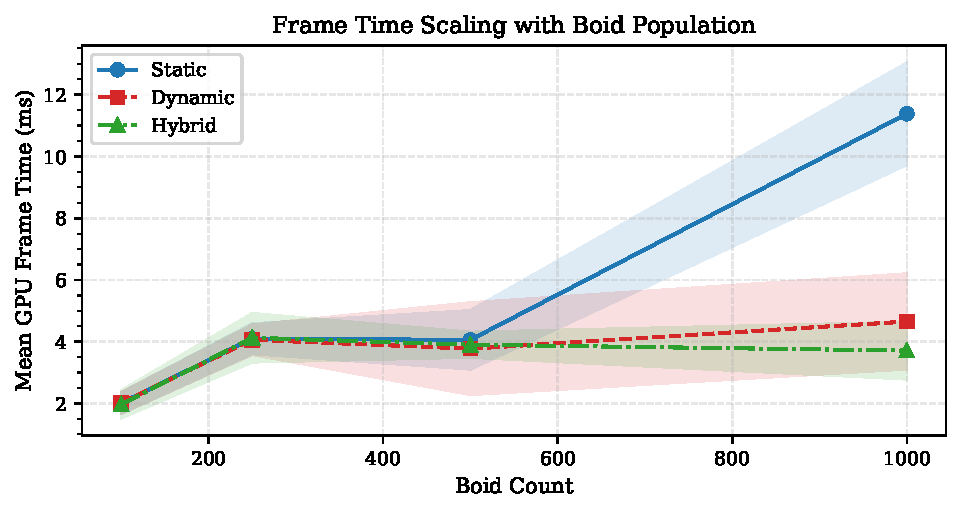
\includegraphics[width=0.55\textwidth]{profiler_scaling.jpg}
  \caption{Mean GPU cost versus boid count across 100, 250, 500, and 1000 agents. Static cost rises steeply beyond 500 boids while Dynamic and Hybrid remain nearly flat.}
  \label{fig:perf-scaling}
\end{figure}

\begin{figure}[H]
  \centering
  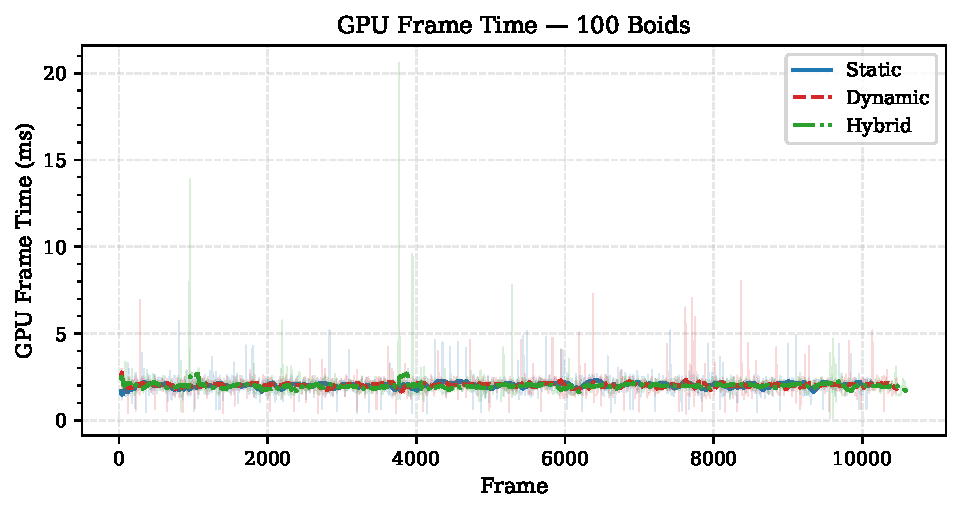
\includegraphics[width=0.55\textwidth]{gpu_timeseries_100.jpg}
  \caption{Frame-by-frame GPU cost for all three configurations at 100 boids.}
  \label{fig:perf-raw}
\end{figure}

\begin{figure}[H]
  \centering
  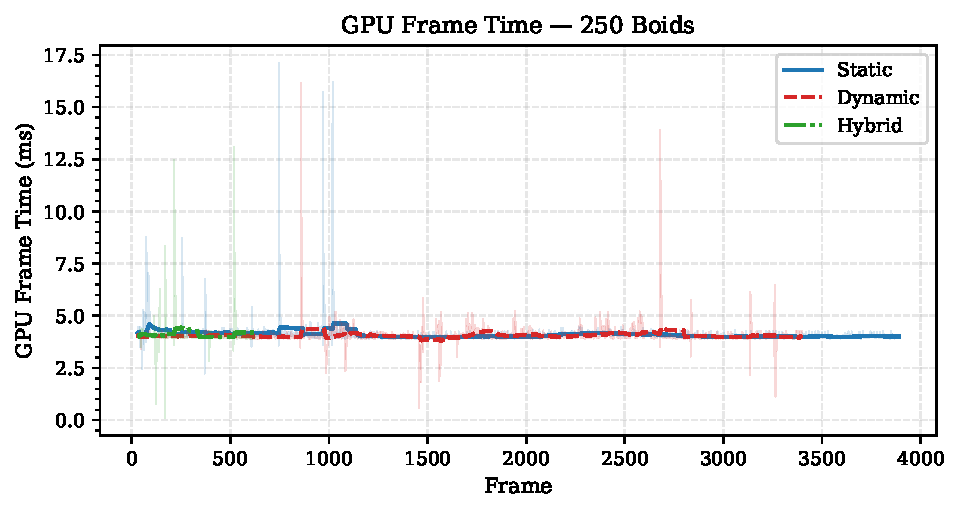
\includegraphics[width=0.55\textwidth]{gpu_timeseries_250.jpg}
  \caption{Frame-by-frame GPU cost for all three configurations at 250 boids.}
  \label{fig:perf-raw}
\end{figure}

\begin{figure}[H]
  \centering
  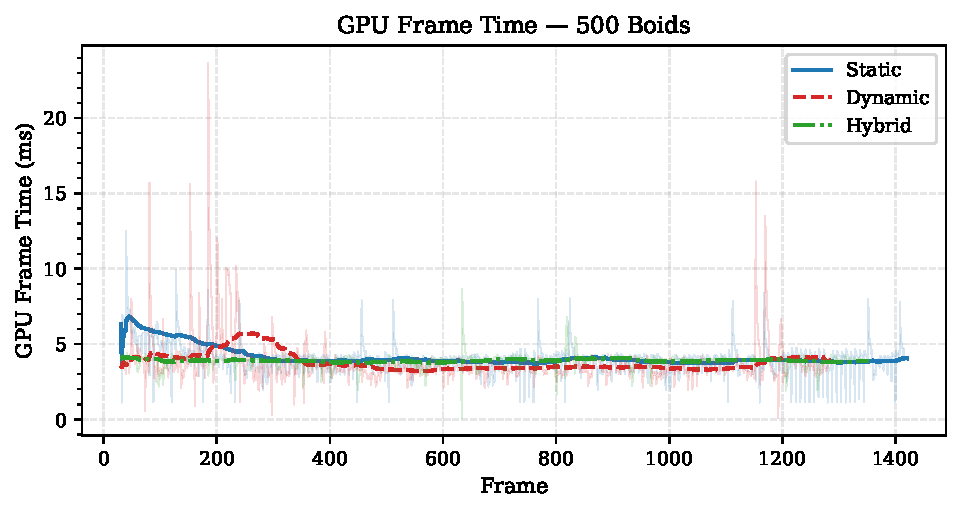
\includegraphics[width=0.55\textwidth]{gpu_timeseries_500.jpg}
  \caption{Frame-by-frame GPU cost for all three configurations at 500 boids.}
  \label{fig:perf-raw}
\end{figure}

\begin{figure}[H]
  \centering
  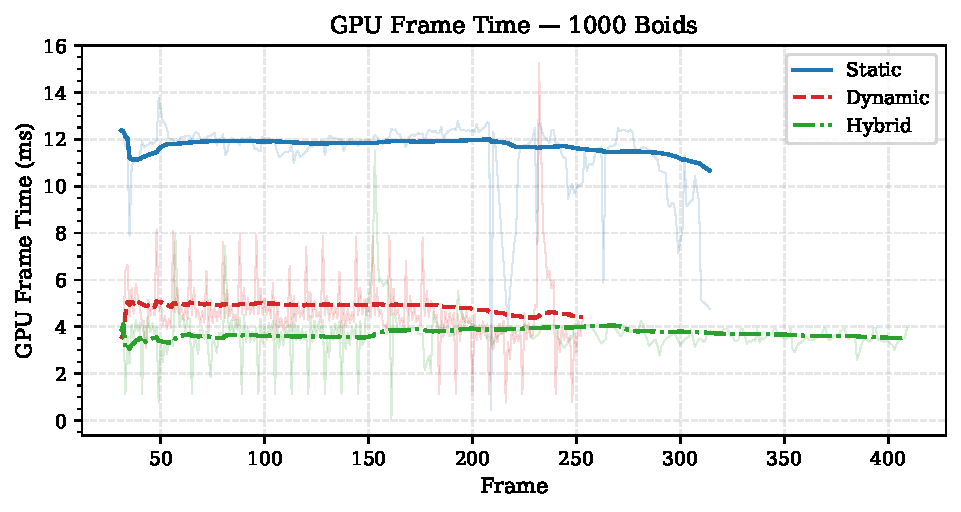
\includegraphics[width=0.55\textwidth]{gpu_timeseries_1000.jpg}
  \caption{Frame-by-frame GPU cost for all three configurations at 1000 boids.}
  \label{fig:perf-raw}
\end{figure}

% \subsection{Image Quality Metrics}

% DSSIM (Structural Dissimilarity) are commonly used to quantitatively measure how effective a rendering technique may be; DSSIM encapsulates information about an object's luminance, structure, and overall fidelity, while LPIPS utilises a pretrained deep network whose feature distances correlate with human perceptual judgements.

\section{Conclusion}
This thesis has demonstrated that a hybrid rendering approach --- assigning the window-panel shader (\texttt{StainedGlassShader.shadergraph}) to the stationary window panel and the lightweight refraction-and-tint shader (\texttt{StainedGlassShaderDynamic.shadergraph}) to GPU-instanced boid agents --- is both technically viable and computationally superior at scale. The performance measurements reported in Section~\ref{sec:performance} show that at low agent counts (100--500 boids) all three configurations perform comparably, but at 1000 boids the hybrid configuration ($3.71\,\text{ms}$) and dynamic configuration ($4.66\,\text{ms}$) both substantially outperform the static configuration ($11.38\,\text{ms}$). The hybrid approach therefore occupies the optimal point in the design space: the UV-mapped source texture in \texttt{StainedGlassShader.shadergraph}, augmented by runtime Spherical Harmonics, Fresnel reflection, and screen-space refraction, preserves the high-frequency visual fidelity of the window panel, while the dynamic boid shader --- using screen-space refraction and texture tinting without a lightmap dependency --- avoids the per-boid fallback lighting overhead that causes the purely static configuration to degrade at scale.

\subsection*{Limitations}

The current implementation is constrained by the low-frequency nature of SH9 lighting in the window-panel shader, which precludes sharp specular highlights on the glass surface. The dynamic boid shader uses screen-space refraction and texture tinting without a lighting model, so boid shards do not receive directional illumination from scene lights. As such, this technique is best suited to enclosed spaces with relatively stable indirect lighting conditions.

\subsection*{Future Research}

Future work could investigate adding Spherical Harmonics evaluation to the dynamic boid shader, giving each agent a spatially-varying ambient lighting contribution without a lightmap dependency. Higher-order SH bases or learnable neural irradiance representations could recover higher-frequency lighting detail for the window-panel shader. Extending the screen-space refraction to support dispersion (wavelength-dependent refraction offsets) would enhance the visual realism of both shaders for coloured glass scenes.

Additionally, work demonstrated in %https://arxiv.org/html/2402.00028v1 
shows that neural networks can be leveraged to further enhance hybrid rendering techniques.

%Mention the neural network hybrid rendering pipelines

% ── REFERENCES ────────────────────────────────────────────────────

\clearpage
\begin{thebibliography}{99}

\bibitem{Green2003}
Robin Green. 2003. Spherical Harmonic Lighting: The Gritty Details.
Presented at the Game Developers Conference (GDC).


\bibitem{Guo2022}
Jie Guo, Zilin Zong, Yanjun Song, Xihao Fu, Chengzhi Tao, Yanwen Guo, and Li-Qian Yan. 2022.
Efficient Light Probes for Real-Time Global Illumination.
\textit{ACM Transactions on Graphics} 41, 6 (2022).
\url{https://doi.org/10.1145/3550454.3555452}

\bibitem{Schied2017}
Christoph Schied, Anton Kaplanyan, Chris Wyman, Anjul Patney,
Chakravarty R.\ Alla Chaitanya, John Burgess, Shiqiu Liu,
Carsten Dachsbacher, Aaron Lefohn, and Marco Salvi. 2017.
Spatiotemporal Variance-Guided Filtering: Real-Time Reconstruction for
Path-Traced Global Illumination.
In \textit{Proceedings of High Performance Graphics (HPG '17)}. ACM.
\url{https://doi.org/10.1145/3105762.3105770}

\bibitem{TanLowChow2024}
Yong Wei Tan, Su Ee Low, Javier Chow, Jeremy Teo, and Anand Bhojan. 2024.
DHR+S: Distributed Hybrid Rendering with Realistic Real-Time Shadows for
Interactive Thin Client Metaverse and Game Applications.
\textit{The Visual Computer} 40 (2024), 4981--4991. Springer.
\url{https://doi.org/10.1007/s00371-024-03501-4}

\bibitem{Reynolds1987}
Craig W. Reynolds. 1987. Flocks, Herds and Schools: A Distributed Behavioral Model.
In \textit{Proceedings of SIGGRAPH '87}, 25--34. ACM.
\url{https://doi.org/10.1145/37401.37406}

\bibitem{Silva2008}
A.\ R.\ Silva \textit{et al.} 2008.
Boids that see: Using self-occlusion for simulating large groups on GPUs.


\bibitem{Mezieres2021}
% TODO: Confirm full citation for the SH ringing artefact paper.
% If the citation cannot be confirmed, remove this entry and the
% \cite{Mezieres2021} reference in Section~2.3.
P.\ M\'ezi\`eres \textit{et al.} 2021.
[Title to be confirmed] --- on ringing artefacts in low-order spherical harmonic lighting.


%https://arxiv.org/html/2402.00028v1

\end{thebibliography}

\end{document}
